\documentclass[11pt]{article}
\usepackage[utf8]{inputenc}
\usepackage[T1]{fontenc}
\usepackage{amsmath,amsfonts,amssymb}
\usepackage{graphicx}
\usepackage{booktabs}
\usepackage{multirow}
\usepackage{url}
\usepackage{xcolor}
\usepackage[numbers,sort&compress]{natbib}
\usepackage[colorlinks=true,citecolor=blue,linkcolor=black,urlcolor=blue]{hyperref}
\usepackage{geometry}
\geometry{margin=1in}

\title{FedMut: Federated Prediction of Combinatorial Mutation Effects Using Pre-trained Protein Language Models}
\author{Bhanvi Paliwal, Caiwei Zhang, Jiayi Zhao, Sihyun Park, Sumeet Kothare, Ushta Samal}
\date{\today}

\begin{document}

\maketitle

\begin{abstract}
Predicting the functional effects of combinatorial mutations is a critical challenge in protein engineering and evolutionary biology. While Deep Mutational Scanning (DMS) provides ground-truth fitness landscapes, the data is often siloed across different institutions and sparse due to the vast combinatorial space of mutations. We present FedMut, a federated learning framework that enables collaborative training of DMS score prediction models across distributed datasets without sharing raw sequence data. Our approach leverages pre-trained protein language models from NVIDIA BioNeMo as feature extractors, combined with a trainable regression head that is optimized using Federated Averaging (FedAvg). We evaluate our method on the ProteinGym Substitution Benchmark, comprising approximately 2.4 million missense variants across 217 DMS assays, partitioned into four federated clients based on biological domain (Human, Virus, Prokaryote, Eukaryote). By freezing the protein language model backbone and only training the prediction head in a federated manner, we hope to reduce communication overhead while maintaining competitive predictive performance. Our framework addresses key challenges in cross-institutional collaboration for protein fitness prediction, enabling privacy-preserving model training that benefits from diverse biological datasets.
\end{abstract}

\section{Summary}

Protein engineering requires accurate prediction of how mutations affect protein function, but experimental data is often distributed across institutions with privacy constraints \cite{Fowler2014}. FedMut addresses this challenge by enabling collaborative machine learning across distributed DMS datasets without sharing raw sequence data \cite{McMahan2017}. Our framework combines pre-trained protein language models from NVIDIA BioNeMo \cite{BioNeMo2024} as frozen feature extractors with locally trainable prediction heads, following the Hydra architecture pattern \cite{Yadan2019Hydra}. This approach allows multiple institutions—such as hospitals, research laboratories, and pharmaceutical companies—to collaboratively improve a shared model while maintaining data privacy and ownership. We demonstrate FedMut on the ProteinGym Substitution Benchmark \cite{Notin2023}, simulating a realistic cross-institutional collaboration with four federated clients representing different biological domains (Human, Virus, Prokaryote, and Eukaryote), enabling privacy-preserving model training that leverages diverse biological datasets.

\subsection{Methods}

FedMut is built using a Hydra architecture \cite{Yadan2019Hydra} that combines a frozen pre-trained protein language model backbone with locally trainable prediction heads, implemented using NVIDIA FLARE \cite{Roth2022} for federated learning orchestration. We evaluate our framework on the ProteinGym Substitution Benchmark \cite{Notin2023}, which comprises approximately 2.4 million missense variants across 217 DMS assays partitioned into four federated clients based on biological domain (Human, Virus, Prokaryote, and Eukaryote) (Table~\ref{tab:clients}). The system architecture consists of a pre-trained BioNeMo model \cite{BioNeMo2024} (e.g., ESM-2 or MegaMolBART) that serves as a frozen feature extractor, taking amino acid sequences as input and producing protein embeddings. On top of this frozen backbone, each federated client adds a lightweight regression head locally, consisting of a pooling layer that aggregates sequence embeddings and a multi-layer perceptron (MLP) that predicts DMS scores. The prediction head is trainable and added locally to each client, allowing for local adaptation while keeping the computationally expensive backbone frozen. During federated training, we employ the Federated Averaging (FedAvg) algorithm \cite{McMahan2017} where the central server initializes prediction head weights and distributes them to all clients. Each client then trains the prediction head on their local data using Mean Squared Error (MSE) loss optimized with AdamW, after which only the updated prediction head weights are sent back to the server for weighted averaging. This process repeats for multiple communication rounds, ensuring that only lightweight prediction head weights are transmitted, significantly reducing communication overhead compared to training the full model.

To use FedMut, institutions first partition their DMS datasets by biological domain and set up federated client nodes, with each client corresponding to a specific taxon. The BioNeMo backbone \cite{BioNeMo2024} is pre-loaded on all clients, and the central server initializes and distributes the prediction head weights. Each client then trains the prediction head locally on their domain-specific data for a specified number of epochs, using the frozen BioNeMo model to extract features from protein sequences. After local training, clients send only their updated prediction head weights to the central server, which performs weighted averaging based on the number of training samples per client. The aggregated global model is then distributed back to all clients for the next round of federated training. This process continues for multiple communication rounds until convergence, enabling collaborative model improvement while preserving data privacy. The resulting federated model can then be used to predict DMS scores for new protein variants, with each client benefiting from the collective knowledge learned across all participating institutions.


\begin{table}[h]
\centering
\caption{Federated client nodes and their simulation scenarios}
\label{tab:clients}
\begin{tabular}{@{}lll@{}}
\toprule
\textbf{Node} & \textbf{Client Type} & \textbf{Simulation Scenario} \\
\midrule
Client 1 & Human & Clinical Hospital / Oncology \\
Client 2 & Virus & Virology Lab / Pandemic Prep \\
Client 3 & Prokaryote & Antibiotic Resistance Lab \\
Client 4 & Eukaryote & Academic Bio-Foundry \\
\bottomrule
\end{tabular}
\end{table}

\begin{figure}[h]
\centering
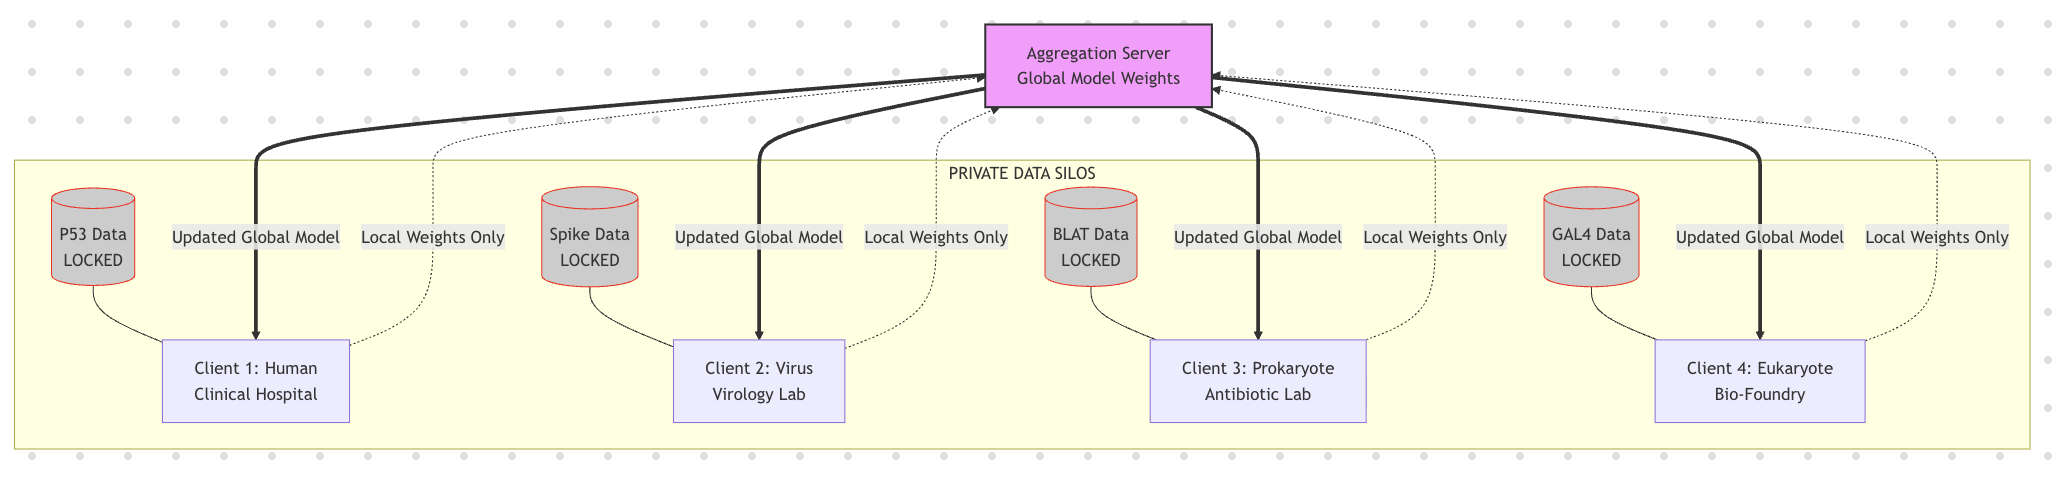
\includegraphics[width=0.8\textwidth]{../figures/clients.png}
\caption{Distribution of DMS assays across federated client nodes based on biological domain.}
\label{fig:clients}
\end{figure}


\section{Results}

\textcolor{red}{[Results section to be filled in with experimental results. Include: evaluation metrics (Spearman's rank correlation, Pearson correlation, MSE, MAE), baseline comparisons (Local Training Only, Centralized Training, Pre-trained Model Only), performance results table across federated clients, and analysis of privacy and communication efficiency.]}

\section{Discussion}

Our FedMut framework addresses critical challenges in collaborative protein fitness prediction by enabling privacy-preserving model training across distributed datasets. The use of frozen pre-trained protein language models as feature extractors provides a practical solution that balances performance, computational efficiency, and communication overhead. The federated learning approach is particularly well-suited for the protein engineering domain, where data is often siloed across institutions due to proprietary interests, regulatory constraints, or competitive advantages. By allowing multiple institutions to collaboratively improve a shared model without sharing raw sequence data, FedMut enables the scientific community to leverage diverse biological datasets while respecting data privacy and ownership.

The partitioning of data by biological domain (Human, Virus, Prokaryote, Eukaryote) creates a realistic non-IID (non-independent and identically distributed) scenario that is common in federated learning applications. This heterogeneity tests the robustness of the FedAvg algorithm and may reveal opportunities for domain-specific adaptations or personalized federated learning approaches. The Hydra architecture, with its frozen backbone and locally trainable heads, offers an efficient compromise between model personalization and communication efficiency, making it particularly suitable for cross-institutional collaboration where computational resources and network bandwidth may be limited.

\subsection{Future Directions}

Several directions for future work are promising. First, systematic hyperparameter optimization for the regression MLP architecture, including layer depth, hidden dimensions, dropout rates, and activation functions, could improve predictive performance. Second, exploration of advanced federated learning algorithms beyond FedAvg, such as FedProx \cite{Li2020} or SCAFFOLD \cite{Karimireddy2020}, may better handle the non-IID data distribution across biological domains and improve convergence rates. Third, extending the framework to multi-task learning, simultaneously predicting both continuous DMS scores and binary fitness classifications, could improve generalization and provide more comprehensive fitness assessments. Additionally, real-world deployment with actual distributed institutions would validate the framework's practicality, addressing challenges such as network latency, client availability, and data quality heterogeneity. Finally, incorporating interpretability methods such as attention visualization or gradient-based techniques could provide biological insights by identifying which sequence regions contribute most to fitness predictions, enhancing both scientific understanding and model trustworthiness.

\section{Conclusion}

FedMut presents a novel federated learning framework for predicting combinatorial mutation effects that addresses key challenges in cross-institutional protein fitness prediction. By combining pre-trained protein language models with federated learning, we enable privacy-preserving collaborative training that can leverage diverse biological datasets while maintaining computational efficiency. Our approach demonstrates the potential for federated learning to advance protein engineering and evolutionary biology research by breaking down data silos and enabling collaborative model development.

\section*{Acknowledgements}

We thank ProteinGym \cite{Notin2023} for providing the benchmarking datasets, NVIDIA BioNeMo for the foundational protein language models, and NVIDIA FLARE \cite{Roth2022} for the federated learning infrastructure. 


\bibliographystyle{plain}
\bibliography{references}

\end{document}
